\documentclass[]{article}
\usepackage{lmodern}
\usepackage{amssymb,amsmath}
\usepackage{ifxetex,ifluatex}
\usepackage{fixltx2e} % provides \textsubscript
\ifnum 0\ifxetex 1\fi\ifluatex 1\fi=0 % if pdftex
  \usepackage[T1]{fontenc}
  \usepackage[utf8]{inputenc}
\else % if luatex or xelatex
  \ifxetex
    \usepackage{mathspec}
  \else
    \usepackage{fontspec}
  \fi
  \defaultfontfeatures{Ligatures=TeX,Scale=MatchLowercase}
\fi
% use upquote if available, for straight quotes in verbatim environments
\IfFileExists{upquote.sty}{\usepackage{upquote}}{}
% use microtype if available
\IfFileExists{microtype.sty}{%
\usepackage[]{microtype}
\UseMicrotypeSet[protrusion]{basicmath} % disable protrusion for tt fonts
}{}
\PassOptionsToPackage{hyphens}{url} % url is loaded by hyperref
\usepackage[unicode=true]{hyperref}
\hypersetup{
            pdftitle={Clasificación de imagenes de radiografias de tórax entre normales y con derrame},
            pdfauthor={Jorge Vallejo Ortega},
            pdfborder={0 0 0},
            breaklinks=true}
\urlstyle{same}  % don't use monospace font for urls
\usepackage[margin=1in]{geometry}
\usepackage{color}
\usepackage{fancyvrb}
\newcommand{\VerbBar}{|}
\newcommand{\VERB}{\Verb[commandchars=\\\{\}]}
\DefineVerbatimEnvironment{Highlighting}{Verbatim}{commandchars=\\\{\}}
% Add ',fontsize=\small' for more characters per line
\usepackage{framed}
\definecolor{shadecolor}{RGB}{248,248,248}
\newenvironment{Shaded}{\begin{snugshade}}{\end{snugshade}}
\newcommand{\KeywordTok}[1]{\textcolor[rgb]{0.13,0.29,0.53}{\textbf{#1}}}
\newcommand{\DataTypeTok}[1]{\textcolor[rgb]{0.13,0.29,0.53}{#1}}
\newcommand{\DecValTok}[1]{\textcolor[rgb]{0.00,0.00,0.81}{#1}}
\newcommand{\BaseNTok}[1]{\textcolor[rgb]{0.00,0.00,0.81}{#1}}
\newcommand{\FloatTok}[1]{\textcolor[rgb]{0.00,0.00,0.81}{#1}}
\newcommand{\ConstantTok}[1]{\textcolor[rgb]{0.00,0.00,0.00}{#1}}
\newcommand{\CharTok}[1]{\textcolor[rgb]{0.31,0.60,0.02}{#1}}
\newcommand{\SpecialCharTok}[1]{\textcolor[rgb]{0.00,0.00,0.00}{#1}}
\newcommand{\StringTok}[1]{\textcolor[rgb]{0.31,0.60,0.02}{#1}}
\newcommand{\VerbatimStringTok}[1]{\textcolor[rgb]{0.31,0.60,0.02}{#1}}
\newcommand{\SpecialStringTok}[1]{\textcolor[rgb]{0.31,0.60,0.02}{#1}}
\newcommand{\ImportTok}[1]{#1}
\newcommand{\CommentTok}[1]{\textcolor[rgb]{0.56,0.35,0.01}{\textit{#1}}}
\newcommand{\DocumentationTok}[1]{\textcolor[rgb]{0.56,0.35,0.01}{\textbf{\textit{#1}}}}
\newcommand{\AnnotationTok}[1]{\textcolor[rgb]{0.56,0.35,0.01}{\textbf{\textit{#1}}}}
\newcommand{\CommentVarTok}[1]{\textcolor[rgb]{0.56,0.35,0.01}{\textbf{\textit{#1}}}}
\newcommand{\OtherTok}[1]{\textcolor[rgb]{0.56,0.35,0.01}{#1}}
\newcommand{\FunctionTok}[1]{\textcolor[rgb]{0.00,0.00,0.00}{#1}}
\newcommand{\VariableTok}[1]{\textcolor[rgb]{0.00,0.00,0.00}{#1}}
\newcommand{\ControlFlowTok}[1]{\textcolor[rgb]{0.13,0.29,0.53}{\textbf{#1}}}
\newcommand{\OperatorTok}[1]{\textcolor[rgb]{0.81,0.36,0.00}{\textbf{#1}}}
\newcommand{\BuiltInTok}[1]{#1}
\newcommand{\ExtensionTok}[1]{#1}
\newcommand{\PreprocessorTok}[1]{\textcolor[rgb]{0.56,0.35,0.01}{\textit{#1}}}
\newcommand{\AttributeTok}[1]{\textcolor[rgb]{0.77,0.63,0.00}{#1}}
\newcommand{\RegionMarkerTok}[1]{#1}
\newcommand{\InformationTok}[1]{\textcolor[rgb]{0.56,0.35,0.01}{\textbf{\textit{#1}}}}
\newcommand{\WarningTok}[1]{\textcolor[rgb]{0.56,0.35,0.01}{\textbf{\textit{#1}}}}
\newcommand{\AlertTok}[1]{\textcolor[rgb]{0.94,0.16,0.16}{#1}}
\newcommand{\ErrorTok}[1]{\textcolor[rgb]{0.64,0.00,0.00}{\textbf{#1}}}
\newcommand{\NormalTok}[1]{#1}
\usepackage{longtable,booktabs}
% Fix footnotes in tables (requires footnote package)
\IfFileExists{footnote.sty}{\usepackage{footnote}\makesavenoteenv{long table}}{}
\usepackage{graphicx,grffile}
\makeatletter
\def\maxwidth{\ifdim\Gin@nat@width>\linewidth\linewidth\else\Gin@nat@width\fi}
\def\maxheight{\ifdim\Gin@nat@height>\textheight\textheight\else\Gin@nat@height\fi}
\makeatother
% Scale images if necessary, so that they will not overflow the page
% margins by default, and it is still possible to overwrite the defaults
% using explicit options in \includegraphics[width, height, ...]{}
\setkeys{Gin}{width=\maxwidth,height=\maxheight,keepaspectratio}
\IfFileExists{parskip.sty}{%
\usepackage{parskip}
}{% else
\setlength{\parindent}{0pt}
\setlength{\parskip}{6pt plus 2pt minus 1pt}
}
\setlength{\emergencystretch}{3em}  % prevent overfull lines
\providecommand{\tightlist}{%
  \setlength{\itemsep}{0pt}\setlength{\parskip}{0pt}}
\setcounter{secnumdepth}{0}
% Redefines (sub)paragraphs to behave more like sections
\ifx\paragraph\undefined\else
\let\oldparagraph\paragraph
\renewcommand{\paragraph}[1]{\oldparagraph{#1}\mbox{}}
\fi
\ifx\subparagraph\undefined\else
\let\oldsubparagraph\subparagraph
\renewcommand{\subparagraph}[1]{\oldsubparagraph{#1}\mbox{}}
\fi

% set default figure placement to htbp
\makeatletter
\def\fps@figure{htbp}
\makeatother

\usepackage{etoolbox}
\makeatletter
\providecommand{\subtitle}[1]{% add subtitle to \maketitle
  \apptocmd{\@title}{\par {\large #1 \par}}{}{}
}
\makeatother

\title{Clasificación de imagenes de radiografias de tórax entre normales y con
derrame}
\providecommand{\subtitle}[1]{}
\subtitle{Machine Learning - PEC 1}
\author{Jorge Vallejo Ortega}
\date{4 de abril, 2020}

\begin{document}
\maketitle

{
\setcounter{tocdepth}{2}
\tableofcontents
}
\section{Índice}\label{uxedndice}

\section{Algoritmo k-NN}\label{algoritmo-k-nn}

El algoritmo de los k vecinos más próximos (\emph{k-nearest neighbours})
es un algoritmo de aprendizaje automático (\emph{machine learning}) que
se utiliza para clasificar observaciones, según si sus características
las hacen más parecidas a uno u otro grupo ya establecidos.

En una primera fase de `entrenamiento', una colección de observaciones
ya clasificadas se distribuyen en un espacio \emph{n}-dimensional. Cada
dimensión corresponde a una de las variables medidas en las
observaciones. Las nuevas observaciones, las cuales queremos clasificar,
se distribuyen a su vez en ese espacio \emph{n}-dimensional; y se
clasifican dentro de los grupos a los que pertenezcan aquellas otras
observaciones, ya clasificadas, de las que más cerca se encuentren. El
número de observaciones conocidas que tenemos en cuenta para clasificar
las observaciones nuevas, es ése número \emph{k}.

\subsection{Fortalezas y debilidades del
algoritmo}\label{fortalezas-y-debilidades-del-algoritmo}

\begin{longtable}[]{@{}ll@{}}
\toprule
Fortalezas & Debilidades\tabularnewline
\midrule
\endhead
*Simple y efectivo & * No produce un modelo, limitando la habilidad para
entender cómo las características se relacionan con la
clasificación\tabularnewline
* No hace asunciones acerca de la distribución subyacente de los datos &
* Requiere seleccionar una \emph{k} adecuada\tabularnewline
* Fase de entrenamiento rápida & * Fase de clasificación
lenta\tabularnewline
& * Se requiere procesado adicional para características nominales y
datos incompletos\tabularnewline
\bottomrule
\end{longtable}

\section{Pre-procesado de datos}\label{pre-procesado-de-datos}

Las imágenes a clasificar deberán estar en una carpeta llamada
``dataset'', en el mismo directorio que el código que vamos a correr.

\begin{Shaded}
\begin{Highlighting}[]
\KeywordTok{dir.create}\NormalTok{(}\StringTok{"./results"}\NormalTok{, }\DataTypeTok{showWarnings =} \OtherTok{FALSE}\NormalTok{)}

\ControlFlowTok{if}\NormalTok{ (}\OperatorTok{!}\StringTok{ }\KeywordTok{dir.exists}\NormalTok{(}\StringTok{"./dataset"}\NormalTok{)) \{}
  \KeywordTok{stop}\NormalTok{(}\StringTok{"El directorio ./dataset no existe"}\NormalTok{)}
\NormalTok{\}}

\CommentTok{# DONE Si datasets existe}
\CommentTok{#    si contiene datos}
\CommentTok{#        Continúa con el script}
\CommentTok{#    else: Aviso (La carpeta datasets no contiene datos)}
\CommentTok{# DONE Else: la carpeta datasets no existe}
\end{Highlighting}
\end{Shaded}

\begin{Shaded}
\begin{Highlighting}[]
\KeywordTok{library}\NormalTok{(}\StringTok{'OpenImageR'}\NormalTok{)}

\NormalTok{image_tovector <-}\StringTok{ }\ControlFlowTok{function}\NormalTok{(x)\{}
\CommentTok{# Create filepath}
\NormalTok{filepath <-}\StringTok{ }\KeywordTok{paste}\NormalTok{(}\StringTok{"./dataset"}\NormalTok{, }\DataTypeTok{sep=}\StringTok{'/'}\NormalTok{,}
                  \KeywordTok{paste}\NormalTok{(}\KeywordTok{as.vector}\NormalTok{(x), }\DataTypeTok{collapse =} \StringTok{'/'}\NormalTok{))}
\CommentTok{#print(filepath)}
\CommentTok{# Read image}
\NormalTok{image <-}\StringTok{ }\KeywordTok{readImage}\NormalTok{(filepath)}
\CommentTok{# Convert to greyscale}
\NormalTok{image_grey <-}\StringTok{ }\KeywordTok{rgb_2gray}\NormalTok{(image)}
\CommentTok{# Resize to 64x64}
\NormalTok{image_resized <-}\StringTok{ }\KeywordTok{resizeImage}\NormalTok{(image_grey, }\DecValTok{64}\NormalTok{, }\DecValTok{64}\NormalTok{)}
\CommentTok{# Transform from matrix to vector}
\KeywordTok{return}\NormalTok{(}\KeywordTok{as.vector}\NormalTok{(image_resized))}
\NormalTok{\}}

\NormalTok{## }\AlertTok{TODO}\NormalTok{ ## Incluir en el informe ejemplos de imagenes antes y después del preprocesado (función imageShow()).}
\end{Highlighting}
\end{Shaded}

\begin{Shaded}
\begin{Highlighting}[]
\NormalTok{directories <-}\StringTok{ }\KeywordTok{list.dirs}\NormalTok{(}\StringTok{"./dataset"}\NormalTok{, }\DataTypeTok{full.names =} \OtherTok{FALSE}\NormalTok{, }\DataTypeTok{recursive =} \OtherTok{FALSE}\NormalTok{)}
\NormalTok{filenames <-}\StringTok{ }\KeywordTok{as.data.frame}\NormalTok{(}
  \KeywordTok{sapply}\NormalTok{(directories,}
                    \ControlFlowTok{function}\NormalTok{ (x)\{}\KeywordTok{return}\NormalTok{(}
                      \KeywordTok{list.files}\NormalTok{(}\KeywordTok{paste0}\NormalTok{(}\StringTok{"./dataset/"}\NormalTok{, x)))\}))}

\CommentTok{# From wide to long format}
\NormalTok{filenames <-}\StringTok{ }\KeywordTok{reshape}\NormalTok{(filenames,}
                      \DataTypeTok{direction=}\StringTok{"long"}\NormalTok{,}
                      \DataTypeTok{varying =} \KeywordTok{c}\NormalTok{(}\StringTok{"effusion"}\NormalTok{, }\StringTok{"normal"}\NormalTok{),}
                      \DataTypeTok{v.names=}\StringTok{"Filename"}\NormalTok{,}
                      \DataTypeTok{timevar=}\StringTok{"cat"}\NormalTok{,}
                      \DataTypeTok{times =} \KeywordTok{c}\NormalTok{(}\StringTok{"effusion"}\NormalTok{, }\StringTok{"normal"}\NormalTok{)}
\NormalTok{                      )}
\KeywordTok{row.names}\NormalTok{(filenames) <-}\StringTok{ }\OtherTok{NULL}
\NormalTok{filenames}\OperatorTok{$}\NormalTok{id <-}\StringTok{ }\OtherTok{NULL}
\CommentTok{#filenames$Condition <- as.factor(filenames$Condition)}
\NormalTok{filenames}\OperatorTok{$}\NormalTok{Filename <-}\StringTok{ }\KeywordTok{as.character}\NormalTok{(filenames}\OperatorTok{$}\NormalTok{Filename)}
\end{Highlighting}
\end{Shaded}

\begin{Shaded}
\begin{Highlighting}[]
\CommentTok{#Check if the file already exists}
\ControlFlowTok{if}\NormalTok{(}\KeywordTok{file.exists}\NormalTok{(}\StringTok{"image_vectors.RData"}\NormalTok{))\{}
  \KeywordTok{load}\NormalTok{(}\StringTok{"image_vectors.RData"}\NormalTok{)}
\NormalTok{\}}\ControlFlowTok{else}\NormalTok{\{}
\CommentTok{# Matrix of vectorized images}
\NormalTok{image_vectors <-}\StringTok{ }\KeywordTok{apply}\NormalTok{(filenames, }\DecValTok{1}\NormalTok{, image_tovector)}
\KeywordTok{save}\NormalTok{(image_vectors, }\DataTypeTok{file =} \StringTok{"image_vectors.RData"}\NormalTok{)}
\NormalTok{\}}
\CommentTok{# This if-else block is to avoid re-calculating }
\CommentTok{# the object every time I want to try the code.}
\CommentTok{# I have just have care to remove the .RData file}
\CommentTok{# if I want to re-calculate it.}

\NormalTok{## }\AlertTok{TODO}\NormalTok{ Keep the file names as col names}

\CommentTok{# Transpose to have images as observations}
\NormalTok{image_vectors <-}\StringTok{ }\KeywordTok{as.data.frame}\NormalTok{(}\KeywordTok{t}\NormalTok{(image_vectors))}
\end{Highlighting}
\end{Shaded}

\begin{Shaded}
\begin{Highlighting}[]
\NormalTok{## How to check if each row if really an x-ray image:}
\NormalTok{test_row <-}\StringTok{ }\ControlFlowTok{function}\NormalTok{(x)\{}
\CommentTok{# Extract one row of the dataframe and store as a numeric vector}
\NormalTok{ test <-}\StringTok{ }\KeywordTok{as.numeric}\NormalTok{(image_vectors[x,])}
\CommentTok{# Transform vector into matrix}
\NormalTok{ test <-}\StringTok{ }\KeywordTok{matrix}\NormalTok{(test, }\DataTypeTok{ncol=}\DecValTok{64}\NormalTok{)}
\CommentTok{# Check if you obtain an x-ray image}
 \KeywordTok{imageShow}\NormalTok{(test)}
\NormalTok{\}}
\end{Highlighting}
\end{Shaded}

\begin{Shaded}
\begin{Highlighting}[]
\NormalTok{image_vectors <-}\StringTok{ }\KeywordTok{cbind}\NormalTok{(filenames, image_vectors)}
\CommentTok{# Change cat variable to factors}
\NormalTok{image_vectors}\OperatorTok{$}\NormalTok{cat <-}\StringTok{ }\KeywordTok{as.factor}\NormalTok{(image_vectors}\OperatorTok{$}\NormalTok{cat)}
\KeywordTok{levels}\NormalTok{(image_vectors}\OperatorTok{$}\NormalTok{cat) <-}\StringTok{ }\KeywordTok{c}\NormalTok{(}\StringTok{"e"}\NormalTok{, }\StringTok{"n"}\NormalTok{)}
\end{Highlighting}
\end{Shaded}

\begin{Shaded}
\begin{Highlighting}[]
\ControlFlowTok{if}\NormalTok{( }\OperatorTok{!}\StringTok{ }\KeywordTok{file.exists}\NormalTok{(}\StringTok{"./results/RX_Torax_4097.csv"}\NormalTok{))\{}
  \KeywordTok{write.csv2}\NormalTok{(image_vectors,}
           \DataTypeTok{file=}\StringTok{"./results/RX_Torax_4097.csv"}\NormalTok{,}
           \DataTypeTok{row.names =} \OtherTok{FALSE}\NormalTok{)}
\NormalTok{\}}

\CommentTok{# Structured in that way to avoid writing the file}
\CommentTok{# each time that I want to test the script,}
\CommentTok{# especially if I just want to test knitting}
\end{Highlighting}
\end{Shaded}

\subsubsection{Lectura de datos}\label{lectura-de-datos}

\begin{Shaded}
\begin{Highlighting}[]
\NormalTok{image_vectors <-}\StringTok{ }\KeywordTok{read.csv2}\NormalTok{(}\StringTok{"./results/RX_Torax_4097.csv"}\NormalTok{)}
\end{Highlighting}
\end{Shaded}

\subsubsection{Estructura de los datos}\label{estructura-de-los-datos}

\begin{Shaded}
\begin{Highlighting}[]
\NormalTok{observaciones <-}\StringTok{ }\KeywordTok{nrow}\NormalTok{(image_vectors)}
\NormalTok{variables <-}\StringTok{ }\KeywordTok{ncol}\NormalTok{(image_vectors)}\OperatorTok{-}\DecValTok{2}
\end{Highlighting}
\end{Shaded}

El set de datos examinado está compuesto por 1000 observaciones, de las
cuales se han tomado 4096 variables, y están divididas en 2 clases
(effusion, normal) that are codified as e, n.

La distribución de cada clase es la siguiente:

\begin{Shaded}
\begin{Highlighting}[]
\KeywordTok{kable}\NormalTok{(}\KeywordTok{table}\NormalTok{(image_vectors}\OperatorTok{$}\NormalTok{cat),}
      \DataTypeTok{col.names =} \KeywordTok{c}\NormalTok{(}\StringTok{"Clase"}\NormalTok{, }\StringTok{"Frecuencia"}\NormalTok{),}
      \DataTypeTok{align =} \KeywordTok{c}\NormalTok{(}\StringTok{'r'}\NormalTok{,}\StringTok{'l'}\NormalTok{))}
\end{Highlighting}
\end{Shaded}

\begin{longtable}[]{@{}rl@{}}
\toprule
Clase & Frecuencia\tabularnewline
\midrule
\endhead
e & 500\tabularnewline
n & 500\tabularnewline
\bottomrule
\end{longtable}

\subsubsection{Histograma de medias}\label{histograma-de-medias}

\begin{Shaded}
\begin{Highlighting}[]
\NormalTok{image_vectors_normal <-}\StringTok{ }\NormalTok{image_vectors[image_vectors}\OperatorTok{$}\NormalTok{cat }\OperatorTok{==}\StringTok{ 'n'}\NormalTok{,]}
\NormalTok{image_vectors_effusion <-}\StringTok{ }\NormalTok{image_vectors[image_vectors}\OperatorTok{$}\NormalTok{cat }\OperatorTok{==}\StringTok{ 'e'}\NormalTok{,]}

\NormalTok{media_normal <-}\StringTok{ }\KeywordTok{apply}\NormalTok{(image_vectors_normal[,}\DecValTok{3}\OperatorTok{:}\KeywordTok{ncol}\NormalTok{(image_vectors_normal)], }\DecValTok{2}\NormalTok{, mean)}
\NormalTok{media_effusion <-}\StringTok{ }\KeywordTok{apply}\NormalTok{(image_vectors_effusion[,}\DecValTok{3}\OperatorTok{:}\KeywordTok{ncol}\NormalTok{(image_vectors_effusion)], }\DecValTok{2}\NormalTok{, mean)}
\end{Highlighting}
\end{Shaded}

\begin{Shaded}
\begin{Highlighting}[]
\NormalTok{sd_normal <-}\StringTok{ }\KeywordTok{apply}\NormalTok{(image_vectors_normal[,}\DecValTok{3}\OperatorTok{:}\KeywordTok{ncol}\NormalTok{(image_vectors_normal)], }\DecValTok{2}\NormalTok{, sd)}
\NormalTok{sd_effusion <-}\StringTok{ }\KeywordTok{apply}\NormalTok{(image_vectors_effusion[,}\DecValTok{3}\OperatorTok{:}\KeywordTok{ncol}\NormalTok{(image_vectors_effusion)], }\DecValTok{2}\NormalTok{, sd)}
\end{Highlighting}
\end{Shaded}

\begin{Shaded}
\begin{Highlighting}[]
\KeywordTok{par}\NormalTok{(}\DataTypeTok{mfrow=} \KeywordTok{c}\NormalTok{(}\DecValTok{1}\NormalTok{,}\DecValTok{2}\NormalTok{))}
\KeywordTok{hist}\NormalTok{(media_normal,}
     \DataTypeTok{main=}\StringTok{"Valor medio de las variables}\CharTok{\textbackslash{}n}\StringTok{Clase normal"}\NormalTok{,}
     \DataTypeTok{ylab =} \StringTok{"Frecuencia"}\NormalTok{,}
     \DataTypeTok{xlab =} \StringTok{"Media"}\NormalTok{,}
     \DataTypeTok{xlim =} \KeywordTok{c}\NormalTok{(}\DecValTok{0}\NormalTok{,}\DecValTok{1}\NormalTok{),}
     \DataTypeTok{ylim =} \KeywordTok{c}\NormalTok{(}\DecValTok{0}\NormalTok{, max_y))}

\KeywordTok{hist}\NormalTok{(media_effusion,}
     \DataTypeTok{main=}\StringTok{"Valor medio de las variables}\CharTok{\textbackslash{}n}\StringTok{Clase effusion"}\NormalTok{,}
     \DataTypeTok{ylab =} \StringTok{"Frecuencia"}\NormalTok{,}
     \DataTypeTok{xlab =} \StringTok{"Media"}\NormalTok{,}
     \DataTypeTok{xlim =} \KeywordTok{c}\NormalTok{(}\DecValTok{0}\NormalTok{,}\DecValTok{1}\NormalTok{),}
     \DataTypeTok{ylim =} \KeywordTok{c}\NormalTok{(}\DecValTok{0}\NormalTok{, max_y))}
\end{Highlighting}
\end{Shaded}

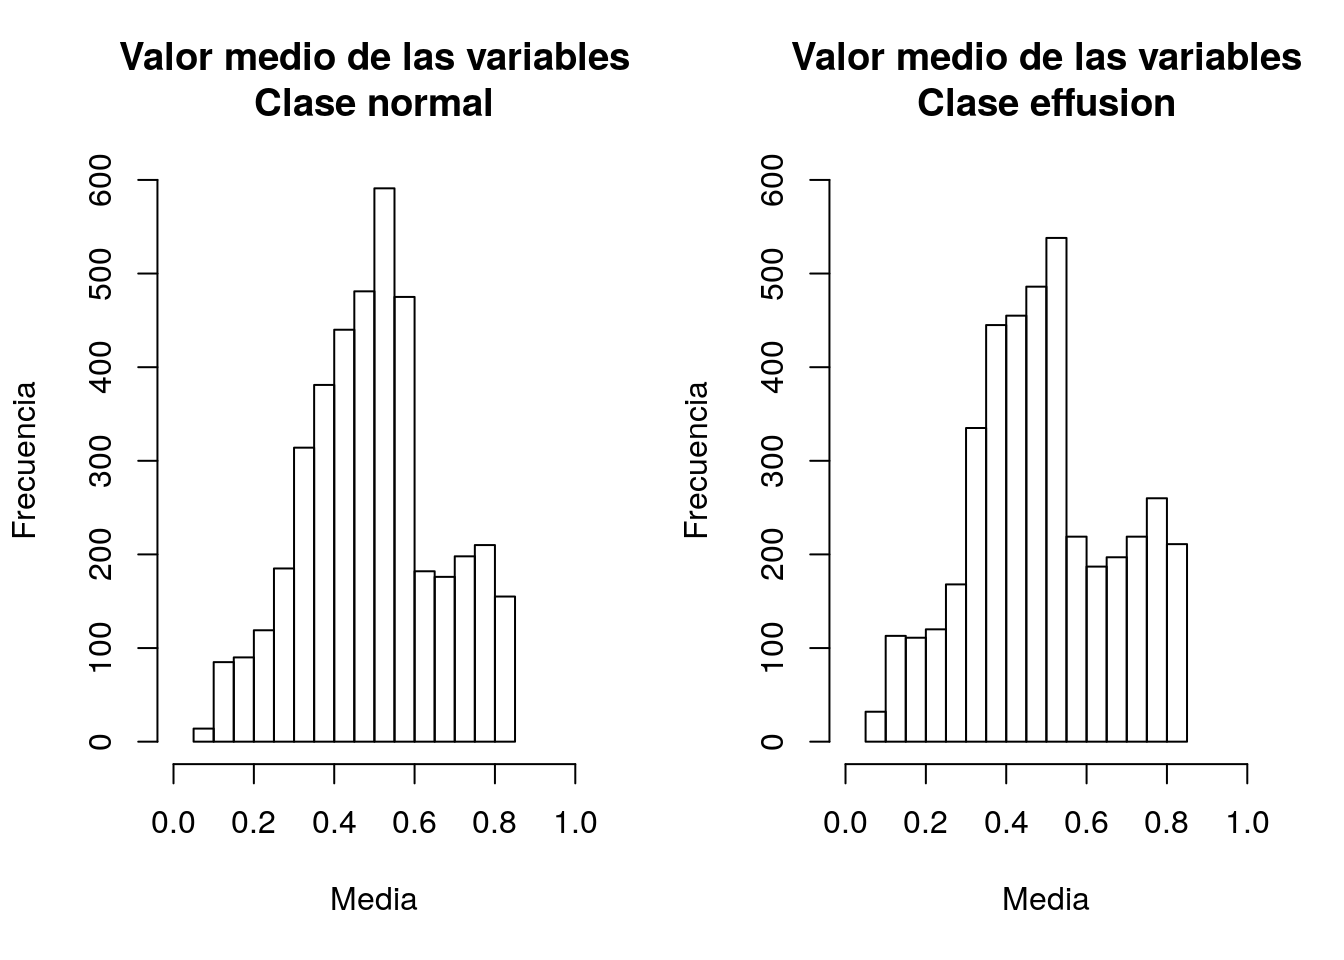
\includegraphics{clasificacion-radiografias_files/figure-latex/histogramas media-1.pdf}

Los valores medios de las variables en la clase ``normal'' parecen estar
más concentrados en el centro de la distribución, mientras que en la
clase ``effusion'' la distribución es más achatada. Esto podría
significar que las imágenes de la clase ``effusion'' presentan áreas más
claras y más oscuras que las imágenes de la clase ``normal''.

\begin{Shaded}
\begin{Highlighting}[]
\KeywordTok{par}\NormalTok{(}\DataTypeTok{mfrow=} \KeywordTok{c}\NormalTok{(}\DecValTok{1}\NormalTok{,}\DecValTok{2}\NormalTok{))}
\KeywordTok{hist}\NormalTok{(sd_normal,}
     \DataTypeTok{main=}\StringTok{"Desviación típica de las variables}\CharTok{\textbackslash{}n}\StringTok{Clase normal"}\NormalTok{,}
     \DataTypeTok{ylab =} \StringTok{"Frecuencia"}\NormalTok{,}
     \DataTypeTok{xlab =} \StringTok{"Media"}\NormalTok{,}
     \DataTypeTok{xlim =} \KeywordTok{c}\NormalTok{(}\DecValTok{0}\NormalTok{,max_xe),}
     \DataTypeTok{ylim =} \KeywordTok{c}\NormalTok{(}\DecValTok{0}\NormalTok{, max_ye))}

\KeywordTok{hist}\NormalTok{(sd_effusion,}
     \DataTypeTok{main=}\StringTok{"Desviación típica de las variables}\CharTok{\textbackslash{}n}\StringTok{Clase effusion"}\NormalTok{,}
     \DataTypeTok{ylab =} \StringTok{"Frecuencia"}\NormalTok{,}
     \DataTypeTok{xlab =} \StringTok{"Desviación típica"}\NormalTok{,}
     \DataTypeTok{xlim =} \KeywordTok{c}\NormalTok{(}\DecValTok{0}\NormalTok{,max_xe),}
     \DataTypeTok{ylim =} \KeywordTok{c}\NormalTok{(}\DecValTok{0}\NormalTok{, max_ye))}
\end{Highlighting}
\end{Shaded}

\includegraphics{clasificacion-radiografias_files/figure-latex/histogramas desviación típica-1.pdf}

Por la forma de los histogramas, y los rangos de valores en los que se
mueven, parece que las variales en las observaciones de clase
``effusion'' presentan valores de desviación típica mayores que las
variables en la clase ``normal''.

\subsection{Contraste de valores medios
(t-test)}\label{contraste-de-valores-medios-t-test}

\begin{Shaded}
\begin{Highlighting}[]
\CommentTok{# Código adaptado de}
\CommentTok{# https://stackoverflow.com/questions/13790611/apply-t-test-on-many-columns-in-a-dataframe-split-by-factor}
\NormalTok{variables_t_test <-}\StringTok{ }\KeywordTok{t}\NormalTok{(}\KeywordTok{sapply}\NormalTok{(image_vectors[}\KeywordTok{c}\NormalTok{(}\OperatorTok{-}\DecValTok{1}\NormalTok{,}\OperatorTok{-}\DecValTok{2}\NormalTok{)], }\ControlFlowTok{function}\NormalTok{(x)}
  \KeywordTok{unlist}\NormalTok{(}\KeywordTok{t.test}\NormalTok{(x}\OperatorTok{~}\NormalTok{image_vectors}\OperatorTok{$}\NormalTok{cat)[}\KeywordTok{c}\NormalTok{(}\StringTok{"estimate"}\NormalTok{, }\StringTok{"p.value"}\NormalTok{)])))}
\end{Highlighting}
\end{Shaded}

\begin{Shaded}
\begin{Highlighting}[]
\NormalTok{variables_t_test_adjusted <-}\StringTok{ }\KeywordTok{as.data.frame}\NormalTok{(variables_t_test)}
\NormalTok{variables_t_test_adjusted[,}\DecValTok{3}\NormalTok{] <-}\StringTok{ }\KeywordTok{p.adjust}\NormalTok{(variables_t_test_adjusted[,}\DecValTok{3}\NormalTok{])}
\CommentTok{# Ordenar los valores de menor a mayor}
\NormalTok{ordered_p_values <-}\StringTok{ }\NormalTok{variables_t_test_adjusted[}\KeywordTok{order}\NormalTok{(variables_t_test[,}\DecValTok{3}\NormalTok{]),]}
\CommentTok{# Añadir columna con diferencia de medias}
\NormalTok{ordered_p_values[, }\StringTok{"diferencia"}\NormalTok{] <-}\StringTok{ }\NormalTok{ordered_p_values[,}\DecValTok{1}\NormalTok{] }\OperatorTok{-}\StringTok{ }\NormalTok{ordered_p_values[,}\DecValTok{2}\NormalTok{]}
\CommentTok{# Preparar para mostrar como tabla}
\KeywordTok{library}\NormalTok{(xtable)}
\KeywordTok{xtable}\NormalTok{(ordered_p_values[}\DecValTok{1}\OperatorTok{:}\DecValTok{25}\NormalTok{,}\OperatorTok{-}\KeywordTok{c}\NormalTok{(}\DecValTok{1}\NormalTok{,}\DecValTok{2}\NormalTok{)],}
       \DataTypeTok{caption =} \StringTok{"Tabla con los 25 descriptores de menor p-valor"}\NormalTok{,}
       \DataTypeTok{digits =} \DecValTok{4}\NormalTok{,}
       \DataTypeTok{display=}\KeywordTok{c}\NormalTok{(}\StringTok{"s"}\NormalTok{, }\StringTok{"e"}\NormalTok{, }\StringTok{"fg"}\NormalTok{))}
\end{Highlighting}
\end{Shaded}

\begin{verbatim}
## % latex table generated in R 3.6.3 by xtable 1.8-4 package
## % Sat Apr  4 20:37:16 2020
## \begin{table}[ht]
## \centering
## \begin{tabular}{rrr}
##   \hline
##  & p.value & diferencia \\ 
##   \hline
## V3052 & 5.2555e-21 & 0.1109 \\ 
##   V3117 & 7.2714e-21 & 0.1128 \\ 
##   V3116 & 1.5192e-20 & 0.1115 \\ 
##   V2989 & 1.7292e-20 & 0.1052 \\ 
##   V1385 & 6.0371e-20 & 0.1162 \\ 
##   V3051 & 6.3355e-20 & 0.1092 \\ 
##   V2988 & 6.4663e-20 & 0.1059 \\ 
##   V1384 & 6.7066e-20 & 0.114 \\ 
##   V2986 & 6.7318e-20 & 0.1065 \\ 
##   V3053 & 6.9608e-20 & 0.1079 \\ 
##   V1387 & 1.0244e-19 & 0.1196 \\ 
##   V2987 & 1.2177e-19 & 0.1048 \\ 
##   V1193 & 1.3655e-19 & 0.1118 \\ 
##   V2924 & 1.7018e-19 & 0.0993 \\ 
##   V1513 & 2.3793e-19 & 0.1128 \\ 
##   V1321 & 3.2334e-19 & 0.1133 \\ 
##   V1256 & 3.6759e-19 &  0.11 \\ 
##   V1192 & 3.9278e-19 & 0.1094 \\ 
##   V2925 & 4.4322e-19 & 0.09896 \\ 
##   V1450 & 4.9911e-19 & 0.1155 \\ 
##   V3050 & 5.1243e-19 & 0.107 \\ 
##   V1451 & 6.6149e-19 & 0.1153 \\ 
##   V1515 & 7.8818e-19 & 0.1136 \\ 
##   V3115 & 8.1534e-19 & 0.107 \\ 
##   V1579 & 9.3589e-19 & 0.1096 \\ 
##    \hline
## \end{tabular}
## \caption{Tabla con los 25 descriptores de menor p-valor} 
## \end{table}
\end{verbatim}

Me llama la atención que en estos descriptores estadísticamente más
significativos, la diferencia entre las medias del grupo ``derrame''" y
del grupo ``normal'' es de alrededor del 20\%.

\subsection{TODO: Normalizar los p-valores ajustados, asociarlos a una
escala de color y reconstruir la imagen para saber qué zonas de la
imagen son más
informativas.}\label{todo-normalizar-los-p-valores-ajustados-asociarlos-a-una-escala-de-color-y-reconstruir-la-imagen-para-saber-quuxe9-zonas-de-la-imagen-son-muxe1s-informativas.}

\subsection{Implementación del algoritmo
knn}\label{implementaciuxf3n-del-algoritmo-knn}

Dividimos el set de datos, al azar, en un set de entrenamiento (67\% de
las observaciones) y un set de prueba (33\% de los datos).

\begin{Shaded}
\begin{Highlighting}[]
\KeywordTok{set.seed}\NormalTok{(}\DecValTok{123}\NormalTok{)}
\CommentTok{# Reordered row numbers}
\NormalTok{observaciones <-}\StringTok{ }\KeywordTok{nrow}\NormalTok{(image_vectors)}
\NormalTok{shuffled_rows <-}\StringTok{ }\KeywordTok{sample}\NormalTok{(observaciones)}
\NormalTok{training_rows <-}\StringTok{ }\NormalTok{shuffled_rows[}\DecValTok{1}\OperatorTok{:}\NormalTok{(observaciones}\OperatorTok{*}\FloatTok{0.67}\NormalTok{)]}
\NormalTok{test_rows <-}\StringTok{ }\NormalTok{shuffled_rows[((observaciones}\OperatorTok{*}\FloatTok{0.67}\NormalTok{)}\OperatorTok{+}\DecValTok{1}\NormalTok{)}\OperatorTok{:}\NormalTok{observaciones]}
\CommentTok{# Remember to use only numeric variables}
\NormalTok{image_vectors_training <-}\StringTok{ }\NormalTok{image_vectors[training_rows, }\DecValTok{3}\OperatorTok{:}\KeywordTok{ncol}\NormalTok{(image_vectors)]}
\NormalTok{image_vectors_test <-}\StringTok{ }\NormalTok{image_vectors[test_rows, }\DecValTok{3}\OperatorTok{:}\KeywordTok{ncol}\NormalTok{(image_vectors)]}

\CommentTok{# Category labels}
\NormalTok{image_vectors_train_labels <-}\StringTok{ }\NormalTok{image_vectors_training[, }\DecValTok{1}\NormalTok{]}
\NormalTok{image_vectors_test_labels <-}\StringTok{ }\NormalTok{image_vectors_test[, }\DecValTok{1}\NormalTok{]}
\end{Highlighting}
\end{Shaded}

\subsection{Evalúa diferentes valores de
k}\label{evaluxfaa-diferentes-valores-de-k}

\begin{Shaded}
\begin{Highlighting}[]
\KeywordTok{library}\NormalTok{(}\StringTok{'class'}\NormalTok{)}
\KeywordTok{library}\NormalTok{(}\StringTok{'gmodels'}\NormalTok{)}

\NormalTok{k <-}\StringTok{ }\KeywordTok{c}\NormalTok{(}\DecValTok{3}\NormalTok{, }\DecValTok{5}\NormalTok{, }\DecValTok{7}\NormalTok{, }\DecValTok{11}\NormalTok{, }\DecValTok{23}\NormalTok{, }\DecValTok{45}\NormalTok{, }\DecValTok{67}\NormalTok{)}

\NormalTok{evaluator <-}\StringTok{ }\ControlFlowTok{function}\NormalTok{ (x)\{}
\NormalTok{  image_vectors_test_pred <-}\StringTok{ }\KeywordTok{knn}\NormalTok{(}\DataTypeTok{train =}\NormalTok{ image_vectors_training,}
                               \DataTypeTok{test =}\NormalTok{ image_vectors_test,}
                               \DataTypeTok{cl =}\NormalTok{ image_vectors_train_labels, }
                               \DataTypeTok{k=}\NormalTok{x)}
\NormalTok{  Results_table <-}\StringTok{ }\KeywordTok{prop.table}\NormalTok{(}
    \KeywordTok{table}\NormalTok{(image_vectors_test_labels,}
\NormalTok{          image_vectors_test_pred))}
  \KeywordTok{return}\NormalTok{(}\KeywordTok{c}\NormalTok{(x, Results_table[}\DecValTok{3}\NormalTok{], Results_table[}\DecValTok{2}\NormalTok{]))}
\NormalTok{\}}

\CommentTok{#Check if the file already exists}
\ControlFlowTok{if}\NormalTok{(}\KeywordTok{file.exists}\NormalTok{(}\StringTok{"./results/evaluated_k.RData"}\NormalTok{))\{}
  \KeywordTok{load}\NormalTok{(}\StringTok{"./results/evaluated_k.RData"}\NormalTok{)}
\NormalTok{\}}\ControlFlowTok{else}\NormalTok{\{}
\CommentTok{# Evaluate the different k values}
\NormalTok{  evaluated_k <-}\StringTok{ }\KeywordTok{sapply}\NormalTok{(k, evaluator)}
  \KeywordTok{save}\NormalTok{(evaluated_k, }\DataTypeTok{file=}\StringTok{"./results/evaluated_k.RData"}\NormalTok{)}
\NormalTok{\}}
\CommentTok{# This if-else block is to avoid re-calculating }
\CommentTok{# the object every time I want to try the code.}
\CommentTok{# I have just have care to remove the .RData file}
\CommentTok{# if I want to re-calculate it.}


\CommentTok{# Format results as a data frame}
\NormalTok{dtevaluated_k <-}\StringTok{ }\KeywordTok{as.data.frame}\NormalTok{(}\KeywordTok{t}\NormalTok{(evaluated_k))}
\CommentTok{# Add column for total errors of classifying}
\NormalTok{dtevaluated_k[,}\DecValTok{4}\NormalTok{] <-}\StringTok{ }\NormalTok{(dtevaluated_k[,}\DecValTok{2}\NormalTok{] }\OperatorTok{+}\StringTok{ }\NormalTok{dtevaluated_k[,}\DecValTok{3}\NormalTok{])}
\CommentTok{# Add column names}
\KeywordTok{colnames}\NormalTok{(dtevaluated_k) <-}\StringTok{ }\KeywordTok{c}\NormalTok{(}\StringTok{"k"}\NormalTok{,}\StringTok{"False Negatives"}\NormalTok{, }\StringTok{"False Positives"}\NormalTok{, }\StringTok{"Total Error"}\NormalTok{)}
\CommentTok{# Format as percentages}
\NormalTok{dtevaluated_k[,}\DecValTok{2}\OperatorTok{:}\DecValTok{4}\NormalTok{] <-}\StringTok{ }\KeywordTok{round}\NormalTok{(dtevaluated_k[,}\DecValTok{2}\OperatorTok{:}\DecValTok{4}\NormalTok{], }\DecValTok{3}\NormalTok{)}\OperatorTok{*}\DecValTok{100}
\NormalTok{dtevaluated_k[,}\DecValTok{2}\OperatorTok{:}\DecValTok{4}\NormalTok{] <-}\StringTok{ }\KeywordTok{mapply}\NormalTok{(paste0, dtevaluated_k[,}\DecValTok{2}\OperatorTok{:}\DecValTok{4}\NormalTok{], }\StringTok{"%"}\NormalTok{)}

\CommentTok{# Print table}
\NormalTok{knitr}\OperatorTok{::}\KeywordTok{kable}\NormalTok{(dtevaluated_k,}
             \DataTypeTok{align =} \KeywordTok{c}\NormalTok{(}\StringTok{"c"}\NormalTok{,}\StringTok{"c"}\NormalTok{,}\StringTok{"c"}\NormalTok{,}\StringTok{"c"}\NormalTok{))}
\end{Highlighting}
\end{Shaded}

\begin{longtable}[]{@{}cccc@{}}
\toprule
k & False Negatives & False Positives & Total Error\tabularnewline
\midrule
\endhead
3 & 0.3\% & 2.4\% & 2.7\%\tabularnewline
5 & 0.6\% & 1.8\% & 2.4\%\tabularnewline
7 & 0\% & 0.9\% & 0.9\%\tabularnewline
11 & 0\% & 0.9\% & 0.9\%\tabularnewline
23 & 0.3\% & 0.9\% & 1.2\%\tabularnewline
45 & 0.9\% & 0.9\% & 1.8\%\tabularnewline
67 & 0.9\% & 1.5\% & 2.4\%\tabularnewline
\bottomrule
\end{longtable}

\end{document}
